\documentclass[twoside]{book}

% Packages required by doxygen
\usepackage{fixltx2e}
\usepackage{calc}
\usepackage{doxygen}
\usepackage[export]{adjustbox} % also loads graphicx
\usepackage{graphicx}
\usepackage[utf8]{inputenc}
\usepackage{makeidx}
\usepackage{multicol}
\usepackage{multirow}
\PassOptionsToPackage{warn}{textcomp}
\usepackage{textcomp}
\usepackage[nointegrals]{wasysym}
\usepackage[table]{xcolor}

% Font selection
\usepackage[T1]{fontenc}
\usepackage[scaled=.90]{helvet}
\usepackage{courier}
\usepackage{amssymb}
\usepackage{sectsty}
\renewcommand{\familydefault}{\sfdefault}
\allsectionsfont{%
  \fontseries{bc}\selectfont%
  \color{darkgray}%
}
\renewcommand{\DoxyLabelFont}{%
  \fontseries{bc}\selectfont%
  \color{darkgray}%
}
\newcommand{\+}{\discretionary{\mbox{\scriptsize$\hookleftarrow$}}{}{}}

% Page & text layout
\usepackage{geometry}
\geometry{%
  a4paper,%
  top=2.5cm,%
  bottom=2.5cm,%
  left=2.5cm,%
  right=2.5cm%
}
\tolerance=750
\hfuzz=15pt
\hbadness=750
\setlength{\emergencystretch}{15pt}
\setlength{\parindent}{0cm}
\setlength{\parskip}{0.2cm}
\makeatletter
\renewcommand{\paragraph}{%
  \@startsection{paragraph}{4}{0ex}{-1.0ex}{1.0ex}{%
    \normalfont\normalsize\bfseries\SS@parafont%
  }%
}
\renewcommand{\subparagraph}{%
  \@startsection{subparagraph}{5}{0ex}{-1.0ex}{1.0ex}{%
    \normalfont\normalsize\bfseries\SS@subparafont%
  }%
}
\makeatother

% Headers & footers
\usepackage{fancyhdr}
\pagestyle{fancyplain}
\fancyhead[LE]{\fancyplain{}{\bfseries\thepage}}
\fancyhead[CE]{\fancyplain{}{}}
\fancyhead[RE]{\fancyplain{}{\bfseries\leftmark}}
\fancyhead[LO]{\fancyplain{}{\bfseries\rightmark}}
\fancyhead[CO]{\fancyplain{}{}}
\fancyhead[RO]{\fancyplain{}{\bfseries\thepage}}
\fancyfoot[LE]{\fancyplain{}{}}
\fancyfoot[CE]{\fancyplain{}{}}
\fancyfoot[RE]{\fancyplain{}{\bfseries\scriptsize Generated on Tue Mar 8 2016 20\+:07\+:54 for Practica2 by Doxygen }}
\fancyfoot[LO]{\fancyplain{}{\bfseries\scriptsize Generated on Tue Mar 8 2016 20\+:07\+:54 for Practica2 by Doxygen }}
\fancyfoot[CO]{\fancyplain{}{}}
\fancyfoot[RO]{\fancyplain{}{}}
\renewcommand{\footrulewidth}{0.4pt}
\renewcommand{\chaptermark}[1]{%
  \markboth{#1}{}%
}
\renewcommand{\sectionmark}[1]{%
  \markright{\thesection\ #1}%
}

% Indices & bibliography
\usepackage{natbib}
\usepackage[titles]{tocloft}
\setcounter{tocdepth}{3}
\setcounter{secnumdepth}{5}
\makeindex

% Hyperlinks (required, but should be loaded last)
\usepackage{ifpdf}
\ifpdf
  \usepackage[pdftex,pagebackref=true]{hyperref}
\else
  \usepackage[ps2pdf,pagebackref=true]{hyperref}
\fi
\hypersetup{%
  colorlinks=true,%
  linkcolor=blue,%
  citecolor=blue,%
  unicode%
}

% Custom commands
\newcommand{\clearemptydoublepage}{%
  \newpage{\pagestyle{empty}\cleardoublepage}%
}


%===== C O N T E N T S =====

\begin{document}

% Titlepage & ToC
\hypersetup{pageanchor=false,
             bookmarks=true,
             bookmarksnumbered=true,
             pdfencoding=unicode
            }
\pagenumbering{roman}
\begin{titlepage}
\vspace*{7cm}
\begin{center}%
{\Large Practica2 }\\
\vspace*{1cm}
{\large Generated by Doxygen 1.8.9.1}\\
\vspace*{0.5cm}
{\small Tue Mar 8 2016 20:07:54}\\
\end{center}
\end{titlepage}
\clearemptydoublepage
\tableofcontents
\clearemptydoublepage
\pagenumbering{arabic}
\hypersetup{pageanchor=true}

%--- Begin generated contents ---
\chapter{Hierarchical Index}
\section{Class Hierarchy}
This inheritance list is sorted roughly, but not completely, alphabetically\+:\begin{DoxyCompactList}
\item \contentsline{section}{Practica4.\+Arbitro}{\pageref{class_practica4_1_1_arbitro}}{}
\item \contentsline{section}{Practica4.\+Pelota}{\pageref{class_practica4_1_1_pelota}}{}
\item Runnable\begin{DoxyCompactList}
\item \contentsline{section}{Practica4.\+Jugador}{\pageref{class_practica4_1_1_jugador}}{}
\end{DoxyCompactList}
\end{DoxyCompactList}

\chapter{Class Index}
\section{Lista de clases}
Lista de las clases, estructuras, uniones e interfaces con una breve descripción\+:\begin{DoxyCompactList}
\item\contentsline{section}{\hyperlink{class_ejercicio1__3__3_1_1_detener___interrupcion}{Ejercicio1\+\_\+3\+\_\+3.\+Detener\+\_\+\+Interrupcion} \\*Thread que se detiene tras una señal del usuario, con diferentes acciones en función del tiempo transcurrido }{\pageref{class_ejercicio1__3__3_1_1_detener___interrupcion}}{}
\item\contentsline{section}{\hyperlink{class_ejercicio1__2__1_1_1_ejercicio1}{Ejercicio1\+\_\+2\+\_\+1.\+Ejercicio1} \\*Creación del número de hilos especificados por el usuario }{\pageref{class_ejercicio1__2__1_1_1_ejercicio1}}{}
\item\contentsline{section}{\hyperlink{class_ejercicio1__2__1_1_1_ejercicio2}{Ejercicio1\+\_\+2\+\_\+1.\+Ejercicio2} \\*Creación del número de hilos especificados por el usuario y medición del tiempo de ejecucion de los hilos }{\pageref{class_ejercicio1__2__1_1_1_ejercicio2}}{}
\item\contentsline{section}{\hyperlink{class_ejercicio1__2__4_1_1_ejercicio4}{Ejercicio1\+\_\+2\+\_\+4.\+Ejercicio4} \\*Cada thread calcula su tiempo de ejecución, lo almacena en una variable publica y se calcula el tiempo total }{\pageref{class_ejercicio1__2__4_1_1_ejercicio4}}{}
\item\contentsline{section}{\hyperlink{class_ejercicio1__2__5_1_1_ejercicio5}{Ejercicio1\+\_\+2\+\_\+5.\+Ejercicio5} \\*Muestra por separados los tiempos de inicialización de threads y los tiempos de ejecución de threads }{\pageref{class_ejercicio1__2__5_1_1_ejercicio5}}{}
\item\contentsline{section}{\hyperlink{class_ejercicio1__2__6_1_1_ejercicio6}{Ejercicio1\+\_\+2\+\_\+6.\+Ejercicio6} \\*Al crear los threads, en caso de introducir el valor \char`\"{}1\char`\"{} se realiza una operación compleja, en caso contrario se procede a la identificación finalización de los threads }{\pageref{class_ejercicio1__2__6_1_1_ejercicio6}}{}
\item\contentsline{section}{\hyperlink{class_ejercicio1__1__2_1_1hello_runnable}{Ejercicio1\+\_\+1\+\_\+2.\+hello\+Runnable} \\*Creación de hilos usando la clase Runnable }{\pageref{class_ejercicio1__1__2_1_1hello_runnable}}{}
\item\contentsline{section}{\hyperlink{class_ejercicio1__1__3_1_1hello_runnable___sleep}{Ejercicio1\+\_\+1\+\_\+3.\+hello\+Runnable\+\_\+\+Sleep} \\*Creación de hilos usando la clase Runnable y usando el método sleep para crear el delay de 1 segundo }{\pageref{class_ejercicio1__1__3_1_1hello_runnable___sleep}}{}
\item\contentsline{section}{\hyperlink{class_ejercicio1__1__2_1_1hello_thread}{Ejercicio1\+\_\+1\+\_\+2.\+hello\+Thread} \\*Creación de hilos usando la clase Thread }{\pageref{class_ejercicio1__1__2_1_1hello_thread}}{}
\item\contentsline{section}{\hyperlink{class_ejercicio1__1__3_1_1hello_thread___sleep}{Ejercicio1\+\_\+1\+\_\+3.\+hello\+Thread\+\_\+\+Sleep} \\*Creación de hilos usando la clase Thread y usando el método sleep para crear el delay de 1 segundo }{\pageref{class_ejercicio1__1__3_1_1hello_thread___sleep}}{}
\item\contentsline{section}{\hyperlink{class_ejercicio1__1__4_1_1_runnable___activo}{Ejercicio1\+\_\+1\+\_\+4.\+Runnable\+\_\+\+Activo} \\*Creación de hilos usando la clase Runnable y usando los metodos active\+Count y current\+Thread para postrar el numero de hilos y el hilo actual }{\pageref{class_ejercicio1__1__4_1_1_runnable___activo}}{}
\item\contentsline{section}{\hyperlink{class_ejercicio1__1__4_1_1_thread___activo}{Ejercicio1\+\_\+1\+\_\+4.\+Thread\+\_\+\+Activo} \\*Creación de hilos usando la clase Thread y usando los metodos active\+Count y current\+Thread para postrar el numero de hilos y el hilo actual }{\pageref{class_ejercicio1__1__4_1_1_thread___activo}}{}
\item\contentsline{section}{\hyperlink{class_ejercicio1__3__2_1_1_thread___detenido}{Ejercicio1\+\_\+3\+\_\+2.\+Thread\+\_\+\+Detenido} \\*Crea un Thread y comprueba con is\+Interrupted() e interrupted() antes y después de interrumpirlo }{\pageref{class_ejercicio1__3__2_1_1_thread___detenido}}{}
\end{DoxyCompactList}

\chapter{Class Documentation}
\hypertarget{class_practica2_1_1_hilos}{}\section{Practica2.\+Hilos Class Reference}
\label{class_practica2_1_1_hilos}\index{Practica2.\+Hilos@{Practica2.\+Hilos}}


Clase que suma los arrays mediante threads, uno para cada fila.  




Inheritance diagram for Practica2.\+Hilos\+:
\nopagebreak
\begin{figure}[H]
\begin{center}
\leavevmode
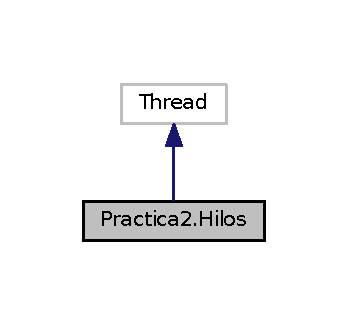
\includegraphics[width=167pt]{class_practica2_1_1_hilos__inherit__graph}
\end{center}
\end{figure}


Collaboration diagram for Practica2.\+Hilos\+:
\nopagebreak
\begin{figure}[H]
\begin{center}
\leavevmode
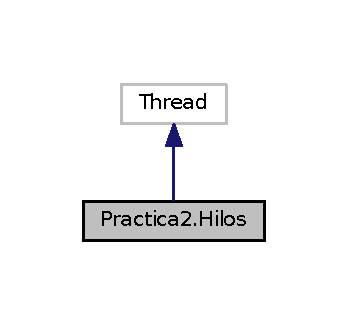
\includegraphics[width=167pt]{class_practica2_1_1_hilos__coll__graph}
\end{center}
\end{figure}
\subsection*{Public Member Functions}
\begin{DoxyCompactItemize}
\item 
\hyperlink{class_practica2_1_1_hilos_a2415cb95146d7a184ee18ffc20e8bbd6}{Hilos} (int n, int f, int fila\+\_\+m1\mbox{[}$\,$\mbox{]}, int fila\+\_\+m2\mbox{[}$\,$\mbox{]})
\begin{DoxyCompactList}\small\item\em Constructor de la Clase, inicializa las variables necesarias y crea el array resultante. \end{DoxyCompactList}\item 
\hypertarget{class_practica2_1_1_hilos_a25701049a60cb68fa20a2b94ecaf01d0}{}void \hyperlink{class_practica2_1_1_hilos_a25701049a60cb68fa20a2b94ecaf01d0}{run} ()\label{class_practica2_1_1_hilos_a25701049a60cb68fa20a2b94ecaf01d0}

\begin{DoxyCompactList}\small\item\em Función run para iniciar el thread, suma ambos arrays y lo almacena en la variable res\mbox{[}\mbox{]}\mbox{[}\mbox{]}, además de calcular su tiempo de ejecución. \end{DoxyCompactList}\end{DoxyCompactItemize}
\subsection*{Static Public Member Functions}
\begin{DoxyCompactItemize}
\item 
static int\mbox{[}$\,$\mbox{]}\mbox{[}$\,$\mbox{]} \hyperlink{class_practica2_1_1_hilos_acf21cb1773256bf75be2bfa3246b5bed}{sumar} (Matriz m1, Matriz m2)
\begin{DoxyCompactList}\small\item\em Función que inicia un thread con cada una de las filas de los arrays y devuelve el array resultante. \end{DoxyCompactList}\item 
\hypertarget{class_practica2_1_1_hilos_a7a6c0033a27bcf745d29a99012114cee}{}static void \hyperlink{class_practica2_1_1_hilos_a7a6c0033a27bcf745d29a99012114cee}{main} (String\mbox{[}$\,$\mbox{]} args)\label{class_practica2_1_1_hilos_a7a6c0033a27bcf745d29a99012114cee}

\begin{DoxyCompactList}\small\item\em Función main del ejercicio, pide que se le introduzca por pantalla el número de elementos del array, crea las matrices a sumar e invoca la función sumar, pasándole como parámetro los arrays creados. \end{DoxyCompactList}\end{DoxyCompactItemize}
\subsection*{Public Attributes}
\begin{DoxyCompactItemize}
\item 
double \hyperlink{class_practica2_1_1_hilos_aaff16bd21f926b0ff36f677f79c87bd7}{tiempo}
\item 
int \hyperlink{class_practica2_1_1_hilos_a90961d2fd4d91c83c8b89fa80f079902}{fm1} \mbox{[}$\,$\mbox{]}
\item 
int \hyperlink{class_practica2_1_1_hilos_aeed8873453657337fb1a6143578e72fb}{fm2} \mbox{[}$\,$\mbox{]}
\end{DoxyCompactItemize}


\subsection{Detailed Description}
Clase que suma los arrays mediante threads, uno para cada fila. 

\begin{DoxyAuthor}{Author}
Nara, Javier, Esteban 
\end{DoxyAuthor}


\subsection{Constructor \& Destructor Documentation}
\hypertarget{class_practica2_1_1_hilos_a2415cb95146d7a184ee18ffc20e8bbd6}{}\index{Practica2\+::\+Hilos@{Practica2\+::\+Hilos}!Hilos@{Hilos}}
\index{Hilos@{Hilos}!Practica2\+::\+Hilos@{Practica2\+::\+Hilos}}
\subsubsection[{Hilos}]{\setlength{\rightskip}{0pt plus 5cm}Practica2.\+Hilos.\+Hilos (
\begin{DoxyParamCaption}
\item[{int}]{n, }
\item[{int}]{f, }
\item[{int}]{fila\+\_\+m1\mbox{[}$\,$\mbox{]}, }
\item[{int}]{fila\+\_\+m2\mbox{[}$\,$\mbox{]}}
\end{DoxyParamCaption}
)}\label{class_practica2_1_1_hilos_a2415cb95146d7a184ee18ffc20e8bbd6}


Constructor de la Clase, inicializa las variables necesarias y crea el array resultante. 


\begin{DoxyParams}{Parameters}
{\em n} & int, el número de filas y columnas que tendrá el array resultante y el número de elementos de los vectores \textquotesingle{}fila\textquotesingle{} \\
\hline
{\em f} & int, el número de fila seleccionado de ambos arrays \\
\hline
{\em fila\+\_\+m1} & int\mbox{[}\mbox{]}, vector con el contenido de una fila de uno de los arrays a sumar \\
\hline
{\em fila\+\_\+m2} & int\mbox{[}\mbox{]}, vector con el contenido de una fila del otro array a sumar \\
\hline
\end{DoxyParams}
\begin{DoxyAuthor}{Author}
Nara, Javier, Esteban 
\end{DoxyAuthor}


\subsection{Member Function Documentation}
\hypertarget{class_practica2_1_1_hilos_acf21cb1773256bf75be2bfa3246b5bed}{}\index{Practica2\+::\+Hilos@{Practica2\+::\+Hilos}!sumar@{sumar}}
\index{sumar@{sumar}!Practica2\+::\+Hilos@{Practica2\+::\+Hilos}}
\subsubsection[{sumar}]{\setlength{\rightskip}{0pt plus 5cm}static int \mbox{[}$\,$\mbox{]}\mbox{[}$\,$\mbox{]} Practica2.\+Hilos.\+sumar (
\begin{DoxyParamCaption}
\item[{Matriz}]{m1, }
\item[{Matriz}]{m2}
\end{DoxyParamCaption}
)\hspace{0.3cm}{\ttfamily [static]}}\label{class_practica2_1_1_hilos_acf21cb1773256bf75be2bfa3246b5bed}


Función que inicia un thread con cada una de las filas de los arrays y devuelve el array resultante. 


\begin{DoxyParams}{Parameters}
{\em m1} & Matriz, elemento que contiene el primer array a sumar \\
\hline
{\em m2} & Matriz, elemento que contiene segundo primer array a sumar \\
\hline
\end{DoxyParams}
\begin{DoxyReturn}{Returns}
res int\mbox{[}\mbox{]}\mbox{[}\mbox{]}, array resultante de la suma de ambos vectores 
\end{DoxyReturn}
\begin{DoxyAuthor}{Author}
Nara, Javier, Esteban 
\end{DoxyAuthor}


\subsection{Member Data Documentation}
\hypertarget{class_practica2_1_1_hilos_a90961d2fd4d91c83c8b89fa80f079902}{}\index{Practica2\+::\+Hilos@{Practica2\+::\+Hilos}!fm1@{fm1}}
\index{fm1@{fm1}!Practica2\+::\+Hilos@{Practica2\+::\+Hilos}}
\subsubsection[{fm1}]{\setlength{\rightskip}{0pt plus 5cm}int Practica2.\+Hilos.\+fm1\mbox{[}$\,$\mbox{]}}\label{class_practica2_1_1_hilos_a90961d2fd4d91c83c8b89fa80f079902}
Filas de la matriz 1 \hypertarget{class_practica2_1_1_hilos_aeed8873453657337fb1a6143578e72fb}{}\index{Practica2\+::\+Hilos@{Practica2\+::\+Hilos}!fm2@{fm2}}
\index{fm2@{fm2}!Practica2\+::\+Hilos@{Practica2\+::\+Hilos}}
\subsubsection[{fm2}]{\setlength{\rightskip}{0pt plus 5cm}int Practica2.\+Hilos.\+fm2\mbox{[}$\,$\mbox{]}}\label{class_practica2_1_1_hilos_aeed8873453657337fb1a6143578e72fb}
Filas de la matriz 2 \hypertarget{class_practica2_1_1_hilos_aaff16bd21f926b0ff36f677f79c87bd7}{}\index{Practica2\+::\+Hilos@{Practica2\+::\+Hilos}!tiempo@{tiempo}}
\index{tiempo@{tiempo}!Practica2\+::\+Hilos@{Practica2\+::\+Hilos}}
\subsubsection[{tiempo}]{\setlength{\rightskip}{0pt plus 5cm}double Practica2.\+Hilos.\+tiempo}\label{class_practica2_1_1_hilos_aaff16bd21f926b0ff36f677f79c87bd7}
Variable tiempo que lleva completar un hilo 

The documentation for this class was generated from the following file\+:\begin{DoxyCompactItemize}
\item 
Hilos.\+java\end{DoxyCompactItemize}

%--- End generated contents ---

% Index
\backmatter
\newpage
\phantomsection
\clearemptydoublepage
\addcontentsline{toc}{chapter}{Index}
\printindex

\end{document}
